\documentclass[a4paper,5pt]{amsbook}
%%%%%%%%%%%%%%%%%%%%%%%%%%%%%%%%%%%%%%%%%%%%%%%%%%%%%%%%%%%%%%%%%%%%%

%\usepackage{booktabs}
\usepackage{graphicx}
%\usepackage{multicol}
%\usepackage{textcomp}
%\usepackage{systeme}
%\usepackage{amssymb}
%\usepackage[]{amsmath}
%\usepackage{subcaption}
\usepackage[inline]{enumitem}
%\usepackage{gensymb}

%%%%%%%%%%%%%%%%%%%%%%%%%%%%%%%%%%%%%%%%%%%%%%%%%%%%%%%%%%%%%%

\newcommand{\sen}{\,\mbox{sen}\,}
\newcommand{\tg}{\,\mbox{tg}\,}
\newcommand{\cosec}{\,\mbox{cosec}\,}
\newcommand{\cotg}{\,\mbox{cotg}\,}
\newcommand{\tr}{\,\mbox{tr}\,}
\newcommand{\ds}{\displaystyle}
\newcommand{\ra}{\rightarrow}

%%%%%%%%%%%%%%%%%%%%%%%%%%%%%%%%%%%%%%%%%%%%%%%%%%%%%%%%%%%%%%%%%%%%%%%%

\setlength{\textwidth}{16cm} \setlength{\topmargin}{-1.7cm}
\setlength{\textheight}{25cm}
\setlength{\leftmargin}{1.2cm} \setlength{\rightmargin}{1.2cm}
\setlength{\oddsidemargin}{0cm}\setlength{\evensidemargin}{0cm}

%%%%%%%%%%%%%%%%%%%%%%%%%%%%%%%%%%%%%%%%%%%%%%%%%%%%%%%%%%%%%%%%%%%%%%%%

% \renewcommand{\baselinestretch}{1.6}
% \renewcommand{\thefootnote}{\fnsymbol{footnote}}
% \renewcommand{\theequation}{\thesection.\arabic{equation}}
% \setlength{\voffset}{-50pt}
% \numberwithin{equation}{chapter}

%%%%%%%%%%%%%%%%%%%%%%%%%%%%%%%%%%%%%%%%%%%%%%%%%%%%%%%%%%%%%%%%%%%%%%%

\begin{document}
\thispagestyle{empty}
\pagestyle{empty}
\begin{minipage}[h]{0.14\textwidth}
	
\includegraphics[scale=0.24]{../../ufgd.png}
\end{minipage}
\begin{minipage}[h]{\textwidth}
\begin{tabular}{c}
{{\bf UNIVERSIDADE FEDERAL DA GRANDE DOURADOS}}\\
{{\bf C\'alculo 2 --- Lista 2}}\\
{{\bf Prof.\ Adriano Barbosa}}\\
\end{tabular}
\vspace{-0.45cm}
%
\end{minipage}

%------------------------

\vspace{1cm}
%%%%%%%%%%%%%%%%%%%%%%%%%%%%%%%%   formulario  inicio  %%%%%%%%%%%%%%%%%%%%%%%%%%%%%%%%
\begin{enumerate}
    \vspace{0.5cm}
    \item Encontre a antiderivada mais geral para as fun\c{c}\~oes abaixo:
        \begin{enumerate}
            \item $f(x)=x-3$
            \item $f(x)=\ds\frac{1}{2}+\frac{3}{4}x^2-\frac{4}{5}x^3$
            \item $f(x)=(x+1)(2x-1)$
            \item $f(x)=\ds\frac{1+x+x^2}{\sqrt{x}}$
            \item $f(x)=2\sen{x}-\sec^2{x}$
        \end{enumerate}

    \vspace{0.5cm}
    \item Encontre $f$ tal que:
        \begin{enumerate}
            \item $f''(x)=20x^3-12x^2+6x$
            \item $f'(x)=1+3\sqrt{x}$, $f(4)=25$
            \item $f'(x)=\sqrt{x}(6+5x)$, $f(1)=10$
            \item $f''(x)=2+\cos{x}$, $f(0)=-1$, $f(\pi/2)=0$
        \end{enumerate}

    \vspace{0.5cm}
    \item O gr\'afico de uma fun\c{c}\~ao $f$ \'e dado em cada item. Determine qual dos
        gr\'aficos $a$, $b$ ou $c$ \'e a antiderivada de $f$.
        \begin{figure}[h]
            \centering
            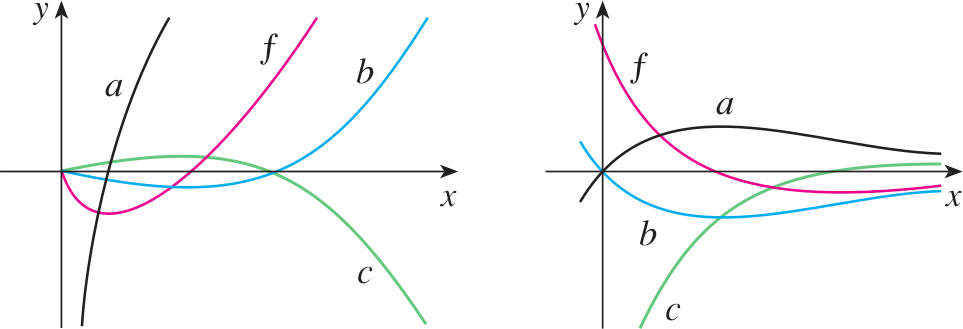
\includegraphics[width=0.6\textwidth]{lista-02-fig1.png}
        \end{figure}

    \vspace{0.5cm}
    \item Como deve ser o gr\'afico de uma antiderivada de $f$ se o gr\'afico de
        $f$ for
        \begin{figure}[h]
            \centering
            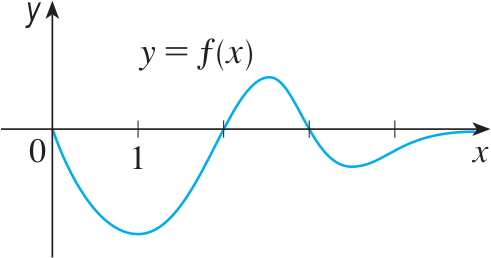
\includegraphics[width=0.3\textwidth]{lista-02-fig2.png}
        \end{figure}

    \vspace{0.5cm}
    \item Use o Teorema Fundamental do C\'alculo para encontrar a derivada das
    	fun\c{c}\~oes abaixo
    \begin{enumerate}
    	\item $\displaystyle g(x) = \int_1^x \frac{1}{t^3 + 1}\ dt$
    	\item $\displaystyle G(x) = \int_x^1 \cos(\sqrt{t})\ dt$
        \item $\displaystyle h(x) = \int_{2x}^{3x} \frac{u^2 - 1}{u^2 + 1}\ du$
            (dica: use as propriedades de integrais e a regra da cadeia.)
    \end{enumerate}

    \vspace{0.5cm}
    \item Calcule as integrais definidas:
    \begin{enumerate}
    	\item $\displaystyle\int_1^2 \frac{3}{t^4}\ dt$
        \vspace{0.3cm}
        \item $\ds\int_0^1 (u+2)(u-3)\ du$
        \vspace{0.3cm}
    	\item $\displaystyle\int_0^{\pi/4} \sec\theta\ \tan\theta\ d\theta$
        \vspace{0.3cm}
    	\item $\displaystyle\int_{-1}^1 e^{u+1}\ du$
        \vspace{0.3cm}
        \item $\ds\int_1^9 \frac{x-1}{\sqrt{x}}\ dx$
        \vspace{0.3cm}
    	\item $\displaystyle\int_0^1 x^e + e^x\ dx$
        \vspace{0.3cm}
    	\item $\displaystyle\int_0^{\pi} f(x)\ dx$, onde $f(x) = \left\{
    			\begin{array}{rl}
    				\sen x, & \mbox{se } 0 \le x < \frac{\pi}{2} \\
    				\cos x, & \mbox{se } \frac{\pi}{2} \le x \le \pi
    			\end{array}\right.$
    \end{enumerate}

    \vspace{0.5cm}
    \item Calcule as integrais indefinidas:
    \begin{enumerate}
        \item $\ds\int x^2+x^{-2}z dx$
        \vspace{0.3cm}
        \item $\ds\int (u+4)(2u+1)\ du$
        \vspace{0.3cm}
        \item $\ds\int \frac{x^2-2\sqrt{x}}{x}\ dx$
        \vspace{0.3cm}
        \item $\ds\int \frac{4+6u}{\sqrt{u}}\ du$
        \vspace{0.3cm}
        \item $\ds\int \sqrt{t}(1+t)\ dt$
        \vspace{0.3cm}
        \item $\ds\int |x-3|\ dx$
    \end{enumerate}
\end{enumerate}

\end{document}
